\documentclass[a4paper]{article}

\usepackage{amsfonts}

\usepackage{tikz}
\usepackage{natbib}
\usepackage{url}
%% Language and font encodings
\usepackage[english]{babel}
\usepackage[utf8x]{inputenc}
\usepackage[T1]{fontenc}

%% Sets page size and margins
\usepackage{fullpage}
%\usepackage[a4paper,top=3cm,bottom=2cm,left=3cm,right=3cm,marginparwidth=1.75cm]{geometry}

%% Useful packages
\usepackage{float}
\usepackage{amsmath}
\usepackage{graphicx}
\usepackage[colorinlistoftodos]{todonotes}
\usepackage[colorlinks=true, allcolors=blue]{hyperref}

\newcommand{\hav}{\text{hav}}
\newcommand{\invhav}{\text{hav}^{-1}}
\title{Visualization using Barnes-Hut algorithm}
\author{Jordan Force}

\begin{document}
\maketitle


\section{Introduction}
I've been working on the visualizations for a few months, and have tried many things that failed. I've learned a lot, and I'd like to document that here, in chronological order. I will explain the idea behind the visualizations, and the different techniques I've tried using to bring those ideas to fruition.

\section{Visualization Idea}

\paragraph{} I'd like to color a map in a way that shows the intensity of storms (especially the economic damage caused by those storms) across the map, across some span of time. My initial plan was to split the map into a grid, and color each cell with a color that represents the amount of economic damage that occured within the cell. However, this has several problems associated with it. First, it creates arbitrary divisions. Second, an extreme storm event may only affect a few cells, even though the results of that storm were catastrophic.  

\paragraph{}Instead, I thought of coloring the storm damage in a way analogous to coloring a surface with the gravitational field on it. For example, this map shows the variation in the gravitational field on the surface of the earth:

\begin{figure}[H]
  \centering
  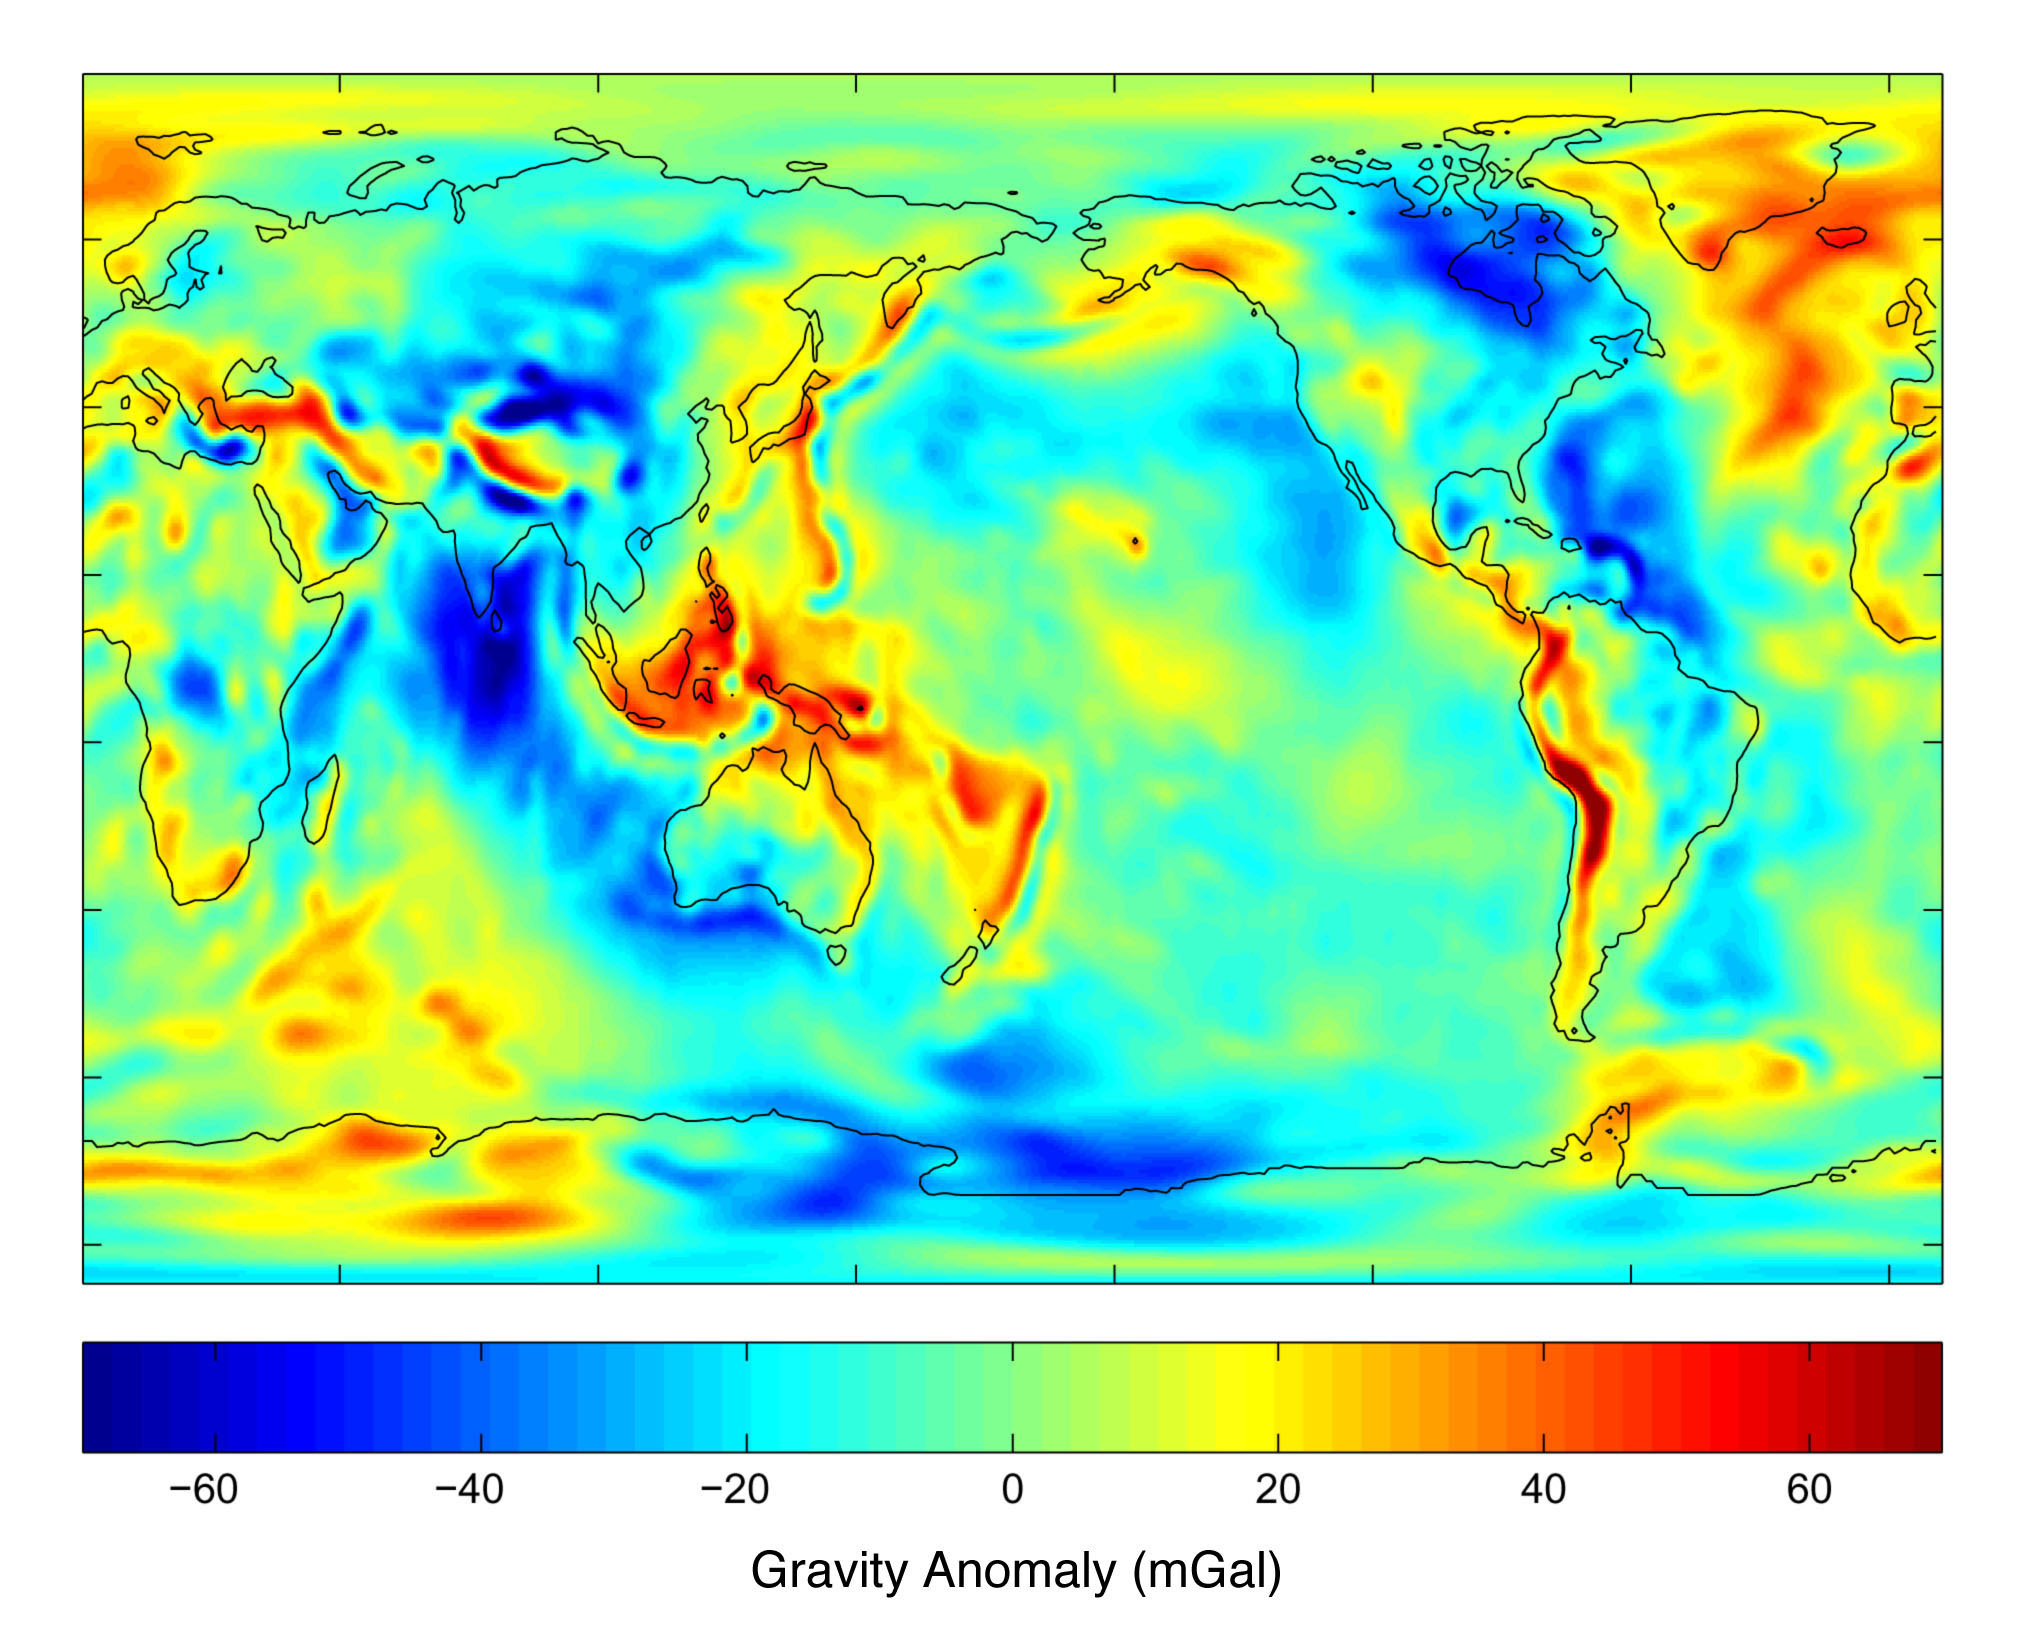
\includegraphics[width=0.77\textwidth]{earth_gravity}
  \caption{Gravitational field. Courtesy of NASA \cite{nasa:gravity}}
\end{figure} 

\paragraph{}There are limitations to this analogy. While a gravitational field is a vector field, our ``field'' would be a scalar field. Suppose you have two point masses on a plane. Each point has the same mass. If you place one point mass at location $(3, 0)$, and the other at location $(-3, 0)$, then the gravitational field at the origin is zero, since a test particle placed at that location would be pulled toward both point masses with the same force, in opposite directions, thus cancelling each other out. Our visualizations should not have this cancelling effect. That is, the ``field'' at a point $(x, y)$ due to $n$ storm events, each with weight $m_{i}$ and at point $(x_{i}, y_{i})$ is:

\begin{equation}
  f(x, y) = \sum_{i = 1}^{n} \dfrac{m_{i}}{\sqrt{(x_{i} - x)^{2} + (y_{i} - y)^{2}}^{2}} = \sum_{i = 1}^{n} \dfrac{m_{i}}{(x_{i} - x)^{2} + (y_{i} - y)^{2}}
\end{equation}

\paragraph{} Of course, this model isn't completely accurate, since earth (despite what some people on the internet might believe) isn't flat. My original plan to deal with this was to project the earth onto a plane, in a very simple manner. Given a set of $n$ points, I calculate the minimum latitude ($\phi_{min}$), maximum latitude ($\phi_{max}$), minimum longitude ($\lambda_{min}$), and maximum longitude ($\lambda_{max}$). I use the two points $(\phi_{min}, \lambda_{min})$ and $(\phi_{min}, \lambda_{max})$ as reference. Let $d$ be the distance between these two points on the earth (I will show how to compute this later). The first point has cartesian location $(0, 0)$, and the second one has cartesian location $(d, 0)$. Given a point $(\phi, \lambda)$, such that $\phi_{min} \leq \phi \leq \phi_{max}$ and $\lambda_{min} \leq \lambda \leq \lambda_{max}$, I would compute the cartesion location using the distance between this point and the reference point at $(0, 0)$, and the distance between this point and the reference point at $(d, 0)$. I won't go through all of the math, but from these distances, I was able to deduce the $x$ and $y$ coordinates of the point. The following figure shows this:


\begin{figure}[H]
\begin{tikzpicture}
  \draw (0,0) node[pos=1.0, left] {$(0, 0)$} -- (4,0) node[pos=1.0, right] {$(d, 0)$} -- (4,4)  -- (0,4) -- (0,0);
  \node at (2, 2.5) {\textbullet};
  \draw (0, 0) -- (2, 2.5) node[midway, above, sloped] {$d_{1}$};
  \draw (2, 2.5) -- (4, 0) node[midway, above, sloped] {$d_{2}$};
\end{tikzpicture}
\centering
\caption{My original projection}
\end{figure}




\paragraph{} To calculate the distance between two points, we use the great circle distance. I originally relied on the definition from Movable Type (known as the Haversine formula)\cite{movableType}, but I am in the process of switching to the definition used in Wolfram Mathematica (as far as I know, the two are equivalent) \cite{wolframHaversine}. We first define the functions:

\begin{equation}
  \text{hav}(z) = \sin^{2}(\dfrac{z}{2})
\end{equation}

\begin{equation}
  \text{hav}^{-1}(z) = 2\sin^{-1}(\sqrt{z})
\end{equation}

Given the Earth's radius $r$, and two points $(\phi_{1}, \lambda_{1}) (\phi_{2}, \lambda_{2})$, the distance between them is:

\begin{equation}
  \label{eq:distance}
  \text{distance}((\phi_{1}, \lambda_{1}), (\phi_{2}, \lambda_{2}), r) = r \text{hav}^{-1}(\text{hav}(\phi_{1} - \phi_{2}) + \cos{\phi_{1}}\cos{\phi_{2}}\text{hav}(\lambda_{1} - \lambda_{2}))
  \end{equation}



\section{Barnes-Hut}
\paragraph{} Coloring in a map would require evaluating the ``field'' at hundreds, thousands, or even hundreds of thousands of points, depending on the resolution. Our database contains millions of storm events. To speed up these computations, I decided to use an algorithm called the barnes-hut algorithm, originally developed for speeding up astrophysics simulations. The basic premise is that clusters of objects, that are sufficiently far away, can be treated as a single object. The barnes-hut algorithm creates a quad-tree by recursively dividing up $\mathbb{R}^{2}$ into quadrants (or $\mathbb{R}^{3}$ into octants), and forming a tree, where the leafs are the actual objects in the tree. The following two images are courtesy of Samzidat Drafting Company:

\begin{figure}[H]
  \centering
  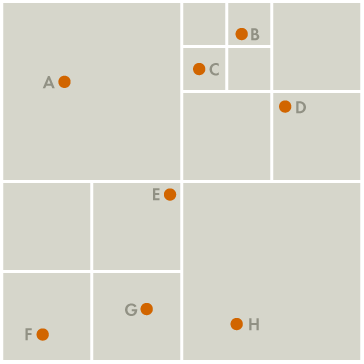
\includegraphics[width=0.5\textwidth]{quadrant}
  \caption{Quadrant being subdivided \cite{barnes_hut}}
\end{figure}   

\begin{figure}[H]
  \centering
  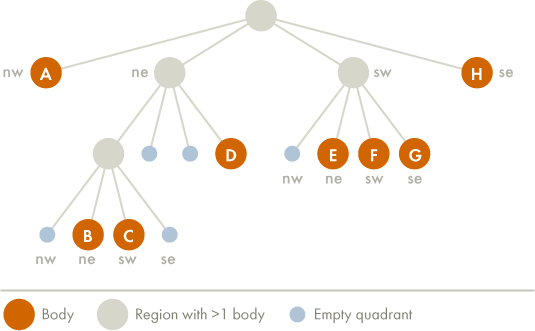
\includegraphics[width=0.77\textwidth]{quadrant_tree}
  \caption{Tree from quadrant subdivision \cite{barnes_hut}}
\end{figure}   

\paragraph{}Each of the internal nodes (colored grey) holds the center of mass of the objects that are children of that internal node. To compute the gravitational field at a point, we traverse the tree, starting from the root, and at each internal node, we let $d$ be the distance from the point to the node's center of mass, and let $s$ be the width of the quadrant that the node represents. If $\dfrac{s}{d} < \theta$, where $\theta$ is some constant (usually $\theta$ is $0.5$), then we use the total mass of objects in the quadrant, and the center of mass, to approximate the field contribution of the child objects. We do not traverse to the children of this internal node.

\paragraph{} My original plan was to take our storm events, project their locations onto a plane, build the barnes-hut tree, and compute the ``field'' at many points, and then project those sampling points back to latitude and longitude coordinates. However, my projection doesn't preserve distances. That is, given two points with distance $d$ between them, it isn't generally the case that the distance between them, when projected onto the cartesian plane, will remain $d$. Actually, there are no isometries (transformations that preserve distance) between the surface of a sphere and a plane \cite{egregium}. Therefore, I need a different plan.


\paragraph{} My current plan is to use the Quadrilaterized Spherical Cube (QSC) projection to project the points onto a plane, and then subdivide that plane into quadrants to create the barnes-hut tree. The QSC projection has the property that a region on the sphere maintains its area when projected using the QSC projection \cite{qsc}. I am using the Proj4 library for doing this projection. Again, since the QSC projection isn't isometric, I need to still work in the latitude and longitude domain when calculating the center of mass for the quadrant. Typically, the center of mass is $R$ such that:

\begin{equation}
  \sum_{i = 1}^{n} m_{i}(\vec{r_{i}} - \vec{R}) = 0
\end{equation}

If I was working in normal cartesian coordinates, I would simply re-arrange the equation to calculate $\vec{R}$. However, there isn't an obvious definition for center of mass on the surface of a sphere. Therefore, I let $\vec{r_{i}} - \vec{R}$ be defined by the initial bearing of the shortest path between $\vec{R}$ and $\vec{r_{i}}$ and the distance of this path. More precisely, we let:

\begin{equation}
  \vec{r_{i}} - \vec{R} = \text{distance}(\vec{r_{i}}, \vec{R}) \begin{bmatrix}
    \cos(\phi_{1})\sin(\phi_{2}) - \sin(\phi_{1})\cos(\phi_{2})\cos(\lambda_{2} - \lambda_{1}) \\
    \sin(\lambda_{2} - \lambda_{1})\cos(\phi_{2})\end{bmatrix}
\end{equation}

Where $\vec{R} = (\phi_{1}, \lambda_{1})$ and $\vec{r_{i}} = (\phi_{2}, \lambda_{2})$, and the distance function is defined in equation \ref{eq:distance}. 

\paragraph{} Unfortunately, there doesn't seem to be a closed form way to compute $\vec{R}$ from this formulation. But, we can use numerical root finding methods to find $\vec{R}$, that get us very close to an exact solution. I've used the Numpy library in Python to achieve this, and I plan on using these methods in my C code using the GNU Scientific Library.


\bibliographystyle{plain}
\bibliography{sources}

\end{document}
